\section{Realisering og test}
\label{realiseringOgTest}

%Her kan du skrive om realisering og test

Figur \ref{fig:Fig2} viser den realiserte løsningen på et overordnet nivå. Telleren som er nevnt i den prinsipielle løsningen er realisert med en adderer som tar inn binære 3-bits tall fra d-vippene i slutten av kretsen og legger det sammen med et fast binært tall. Deretter går signalet inn i en 3-bit mux med to innganger, som vil resete kretsen til 001 dersom signalet blir 110. D-vippene lagrer dataen og sender det nåværende tallet tilbake til addereren og starter kretsen på nytt. Med denne oppkoblingen er det klokken til d-vippen som bestemmer hvor raskt telleren teller. Deretter er det et register med d-vipper som lagrer verdien til telleren ved en stigenede flanke og på den måten lagre et tilfeldig tall fra telleren og sende det videre til dekoderen.Dekoderen tar inn et 3-bit signal og bestemmer hvilke LEDs i matrisen som skal lyse.

\begin{figure}[htbp]
  \centering
  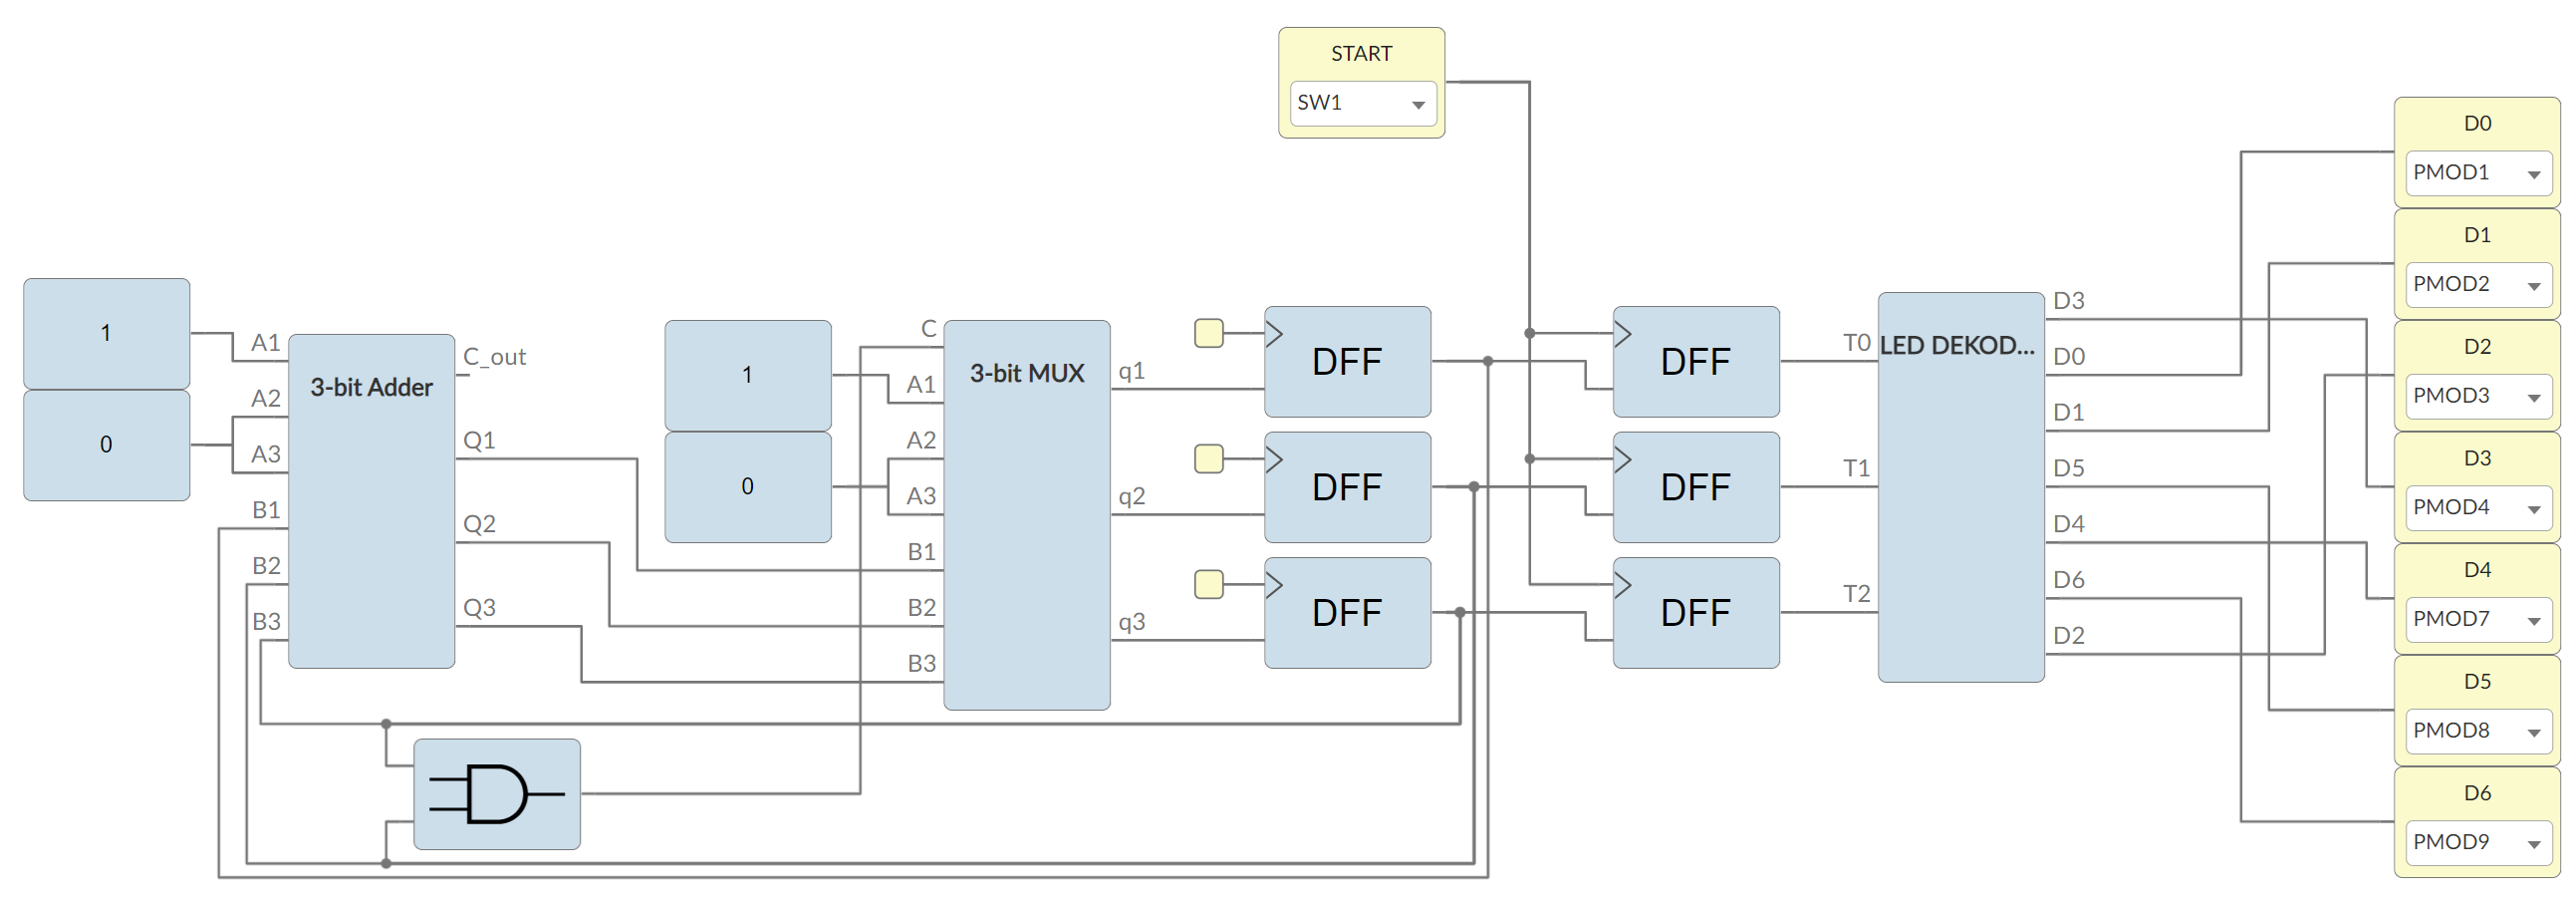
\includegraphics[width=0.6\textwidth]{Bilder/Realisert.png} 
  \caption{Overblikk over den realiserte kretsen}
  \label{fig:Fig2}
\end{figure}


Figur \ref{fig:Fig3} viser realiseringen av en 3-bits fulladderer. 